\section{Experiments}
\begin{table}[t]
  \centering
  \vspace{8pt}
  \tabcolsep=0.11cm{
  \begin{tabular}{ccccc}
    \toprule[1.5pt]
      \textbf{\# Objects} & \textbf{System} & \textbf{\% Solved (SD)} & \textbf{Avg Ref Time (s)} & \textbf{Avg \# MP Calls}\\
    \midrule[2pt]
      30 (can) & T & 42 (0) & 6.2 & 8.0\\
    \midrule
      30 (can) & B & 40 (0) & 20.5 & 10.5\\
    \midrule
      30 (can) & L & 72 (8.2) & 20.4 & 11.3\\
    \midrule
      30 (can) & F & 81 (3.0) & 17.9 & 12.7\\
    \midrule[1.5pt]
      35 (can) & T & 50 (0) & 9.2 & 8.0\\
    \midrule
      35 (can) & B & 50 (0) & 17.6 & 9.2\\
    \midrule
      35 (can) & L & 68 (8.3) & 11.6 & 6.6\\
    \midrule
      35 (can) & F & 78 (2.2) & 10.6 & 6.8\\
    \midrule[1.5pt]
      40 (can) & T & 34 (0) & 19.7 & 10.3\\
    \midrule
      40 (can) & B & 36 (0) & 21.7 & 10.0\\
    \midrule
      40 (can) & L & 61 (6.3) & 18.7 & 9.4\\
    \midrule
      40 (can) & F & 74 (3.2) & 20.7 & 10.4\\
    \midrule[2pt]
      2 (dinner) & T & 100 (0) & 35.5 & 60.2\\
    \midrule
      2 (dinner) & B & 100 (0) & 37.3 & 59.2\\
    \midrule
      2 (dinner) & L & 99 (1.8) & 41.5 & 61.6\\
    \midrule[1.5pt]
      4 (dinner) & T & 100 (0) & 43.2 & 98.0\\
    \midrule
      4 (dinner) & B & 90 (0) & 63.0 & 95.5\\
    \midrule
      4 (dinner) & L & 99 (0.6) & 69.2 & 97.1\\
    \midrule[2pt]
      2 (frying) & T & 96 (0) & 29.0 & 67.2\\
    \midrule
      2 (frying) & B & 88 (0) & 46.9 & 60.0\\
    \midrule
      2 (frying) & L & 99 (2.0) & 22.6 & 44.7\\
    \midrule[1.5pt]
      4 (frying) & T & 55 (0) & 48.9 & 131.8\\
    \midrule
      4 (frying) & B & 20 (0) & 187.9 & 155.5\\
    \midrule
      4 (frying) & L & 92 (6.8) & 90.6 & 120.9\\
    \bottomrule[1.5pt]
  \end{tabular}}
  \caption{\small{Percent solved and standard deviation, along with time spent refining and number of calls to the motion
planner for baseline 1 (T), baseline 2 (B), our learned refinement policies with the graph search used in baseline 2 (L),
and our full system: learned refinement policies and graph search heuristics (F). Results for L and F
are averaged across 5 separately trained sets of weights. As described, we only run F for the can domain. Time limit: 300s.}}
  \label{table:results}
  \vspace{-1em}
\end{table}

\subsection{Methodology}
For refinement distributions, initial experimentation revealed that training weights for all reference types jointly is intractable,
because planning takes a long time. Potential solutions for this would explore alternative {\sc rl} algorithms,
but this is not our focus. Instead, we apply curriculum learning by training with a planning problem distribution
$\Prob$ that gets progressively harder. The details of this curriculum are described in each experiment's section.
Additionally, we train the refinement policies first, then fix them while collecting demonstrations and training the graph search heuristics.

We evaluate our approach in three distinct domains: cans distributed randomly on a table (the \emph{can domain}),
setting up bowls for dinner (the \emph{dinner domain}), and placing frying pans into a narrow shelf (the \emph{frying domain}).
We compare performance with two baselines, both of which use the hand-coded refinement distributions used in {\sc sfrcra-14}.

Baseline 1 is {\sc sfrcra-14}: it uses exhaustive backtracking search for refinement
and greedy depth-first search of the plan refinement graph, which always tries to refine
the plan that incorporates all error information obtained thus far.
Baseline 2 uses randomized refinement with the following fixed graph search policy: try 3 times to refine the deepest
node in the graph; if unsuccessful, generate a geometric fact from it, replan with the task planner (which creates a child node), and repeat.

For the can domain, we report results for 4 systems: 1) baseline 1; 2) baseline 2; 3) our learned refinement policies
with the graph search used in baseline 2; and 4) our full system, with learned refinement policies and graph search heuristics.
For the dinner domain and frying domain, we report results only for the first 3 systems, because the errors propagated in these
domains relate to the stackability of objects. Since this is independent of the current refinement, we want to
incorporate all available error information when attempting refinement. Thus, the graph search strategy
from baseline 2 can be expected to perform well in these settings.

We employ the following algorithm to produce a trained set of weights $\theta_{p}$ for refinement. We train 3 sets independently,
test each one on a validation set, and output the best-performing one. We found that this
reduced variation due to random seeding. The step size $\alpha$ was set to 0.1.

We report results on fixed test sets of 50 randomly generated environments for the can and dinner domains,
and 20 for the frying domain (because the frying domain environments do not have as much variation).
For the third and fourth systems, we average results across running the training
process 5 times independently and evaluating each final set of weights. To train the graph search heuristics,
we collect approximately 300 optimal actions from the human demonstrator, over 3 rounds of {\sc DAgger}. After these 3 rounds,
we found that performance plateaued. We used $C = 10^{9}$ and constant margin $d = 1$ in solving the optimization.

Our experiments are conducted in Python 2.7 using the OpenRave simulator~\cite{Diankov_2008_6117} with a PR2 robot.
The motion planner we use is trajopt~\cite{schulman2013finding}, and the task planner is Fast-Forward~\cite{FF}.
The experiments were carried out in series on an Intel Core i7-4770K machine with 16GB RAM.
Table \ref{table:results} summarizes our quantitative results.

\begin{figure}[t]
  \centering
  \begin{subfigure}[b]{0.35\linewidth}
    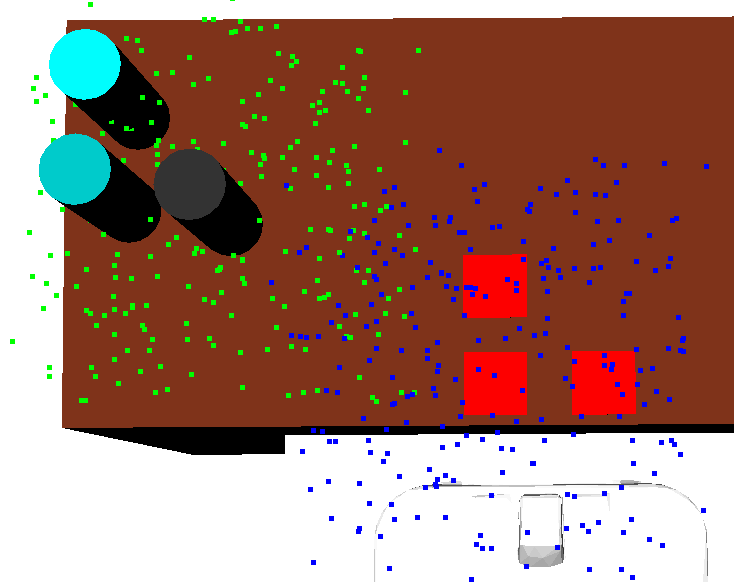
\includegraphics[width=\textwidth]{images/learns.png}
    \caption{Initial distributions.}
  \end{subfigure}
  \begin{subfigure}[b]{0.35\linewidth}
    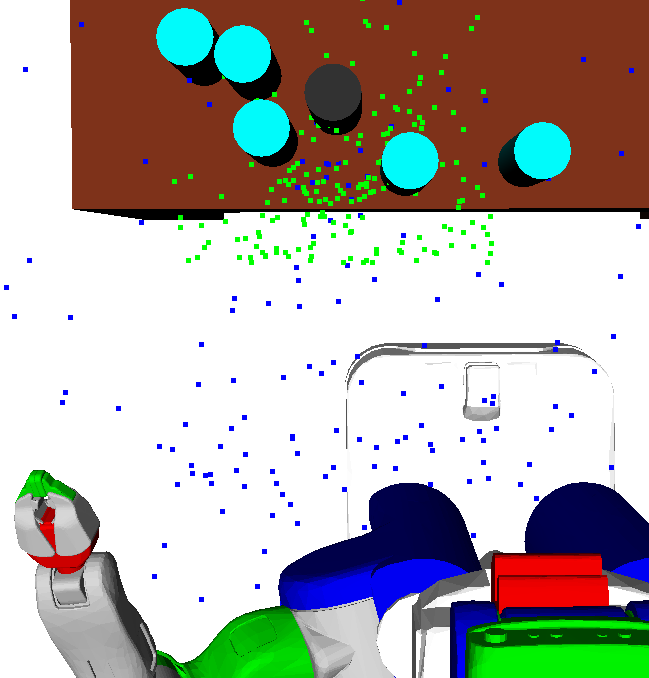
\includegraphics[width=\textwidth]{images/learn4.png}
    \caption{After 4 iterations.}
  \end{subfigure}
  \begin{subfigure}[b]{0.35\linewidth}
    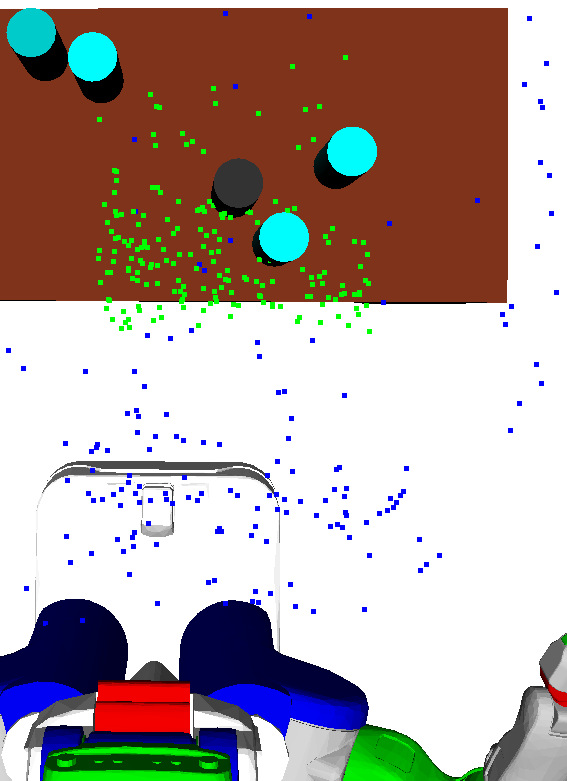
\includegraphics[width=\textwidth]{images/learn8.png}
    \caption{After 8 iterations.}
  \end{subfigure}
  \begin{subfigure}[b]{0.35\linewidth}
    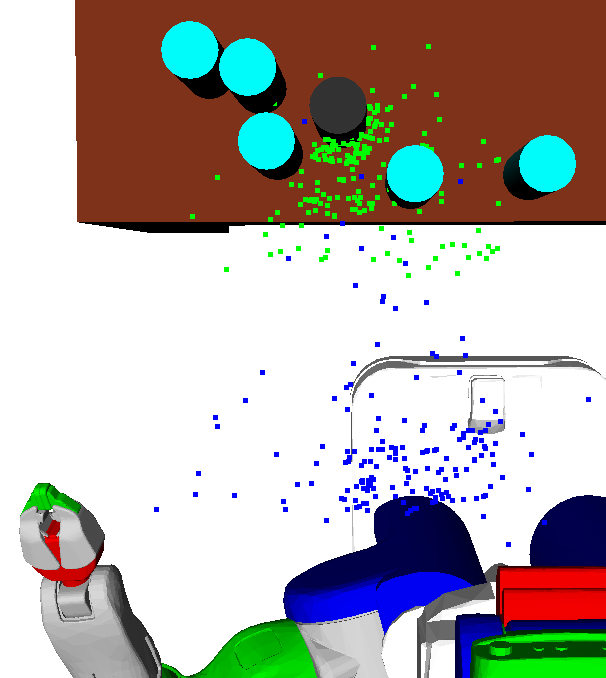
\includegraphics[width=\textwidth]{images/learn12.png}
    \caption{Final distributions.}
  \end{subfigure}
  \caption{\small{Learned base position (blue) and left arm grasp (green) distributions used to
pick up the black can after different training iterations for learning refinement policies.
An iteration refers to a single planning problem,
which terminates after $H$ calls to the \textsc{Resample} routine.
Initial distributions are uniform because we initialize weights to $\vec{\mathbf{0}}$.
Final distributions are after 12 iterations.}}
  \label{fig:training}
\end{figure}

\begin{figure}[t]
  \centering
    \noindent
    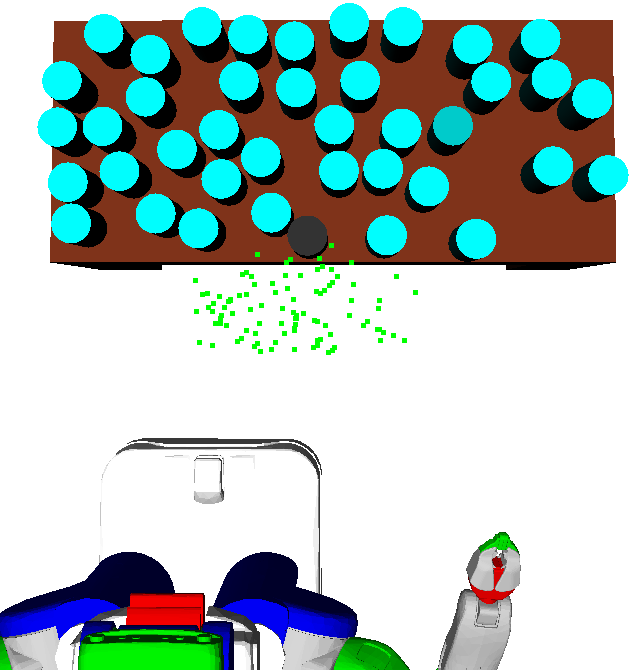
\includegraphics[scale=0.15]{images/grasp_context_left.png}\hspace{6mm}
    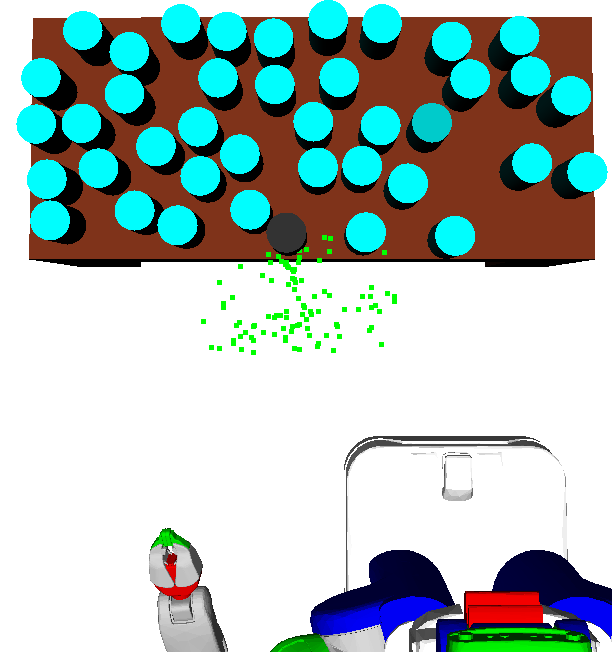
\includegraphics[scale=0.15]{images/grasp_context_right.png}
  \caption{\small{The learned left arm grasp (green) distribution is affected slightly
by relative robot location.}}
  \label{fig:context}
\end{figure}

\subsection{Can Domain}
We run three sets of experiments, using 30, 35, and 40 cans on the table.
The goal is always for the robot to pick up a particular can with its
left gripper. We disabled the right gripper, so any obstructions to the target object must be picked up and
placed elsewhere on the table. This domain has 4 types of continuous references: base poses, object grasp
poses, object putdown poses, and object putdown locations.
% The range of allowable values for grasp and putdown poses is a cube of side length 30 centimeters around the
% target object or putdown location. For base poses, the range is a square of side length 1 meter around the
% object or location which the robot is approaching. For putdown locations, the range is defined by the table.

Our curriculum learning system first trains base poses and grasp poses for $N = 12$ iterations with $\epsilon = 5$,
then base poses, grasp poses, and putdown poses (at fixed location) for $N = 18$ iterations with $\epsilon = 20$,
then all reference types for $N = 30$ iterations with $\epsilon = 20$. We fixed $H = 100$.

The results demonstrate significant improvements in performance to the baseline systems for success rate.
However, backtracking search provides faster average refinement time. This is likely because
refinement times were averaged over the test cases where all 4 systems succeeded. These plans tended
to be easier to refine, so exhaustive backtracking search performs well because the total search space is small.
\figref{fig:cover} and \figref{fig:training} show learned refinement distributions. \figref{fig:context} shows
that our system learned to shape distributions based on the ``context'' in which an action is performed.

\begin{figure}[t]
  \centering
  \begin{subfigure}[b]{0.45\linewidth}
    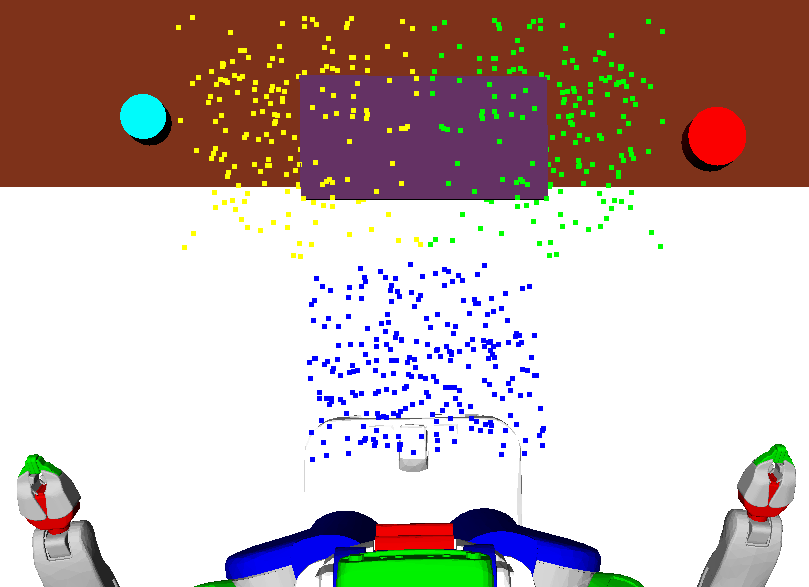
\includegraphics[width=\textwidth]{images/dinner_tray_initial.png}
    \caption{Initial distributions.}
  \end{subfigure}
  \begin{subfigure}[b]{0.45\linewidth}
    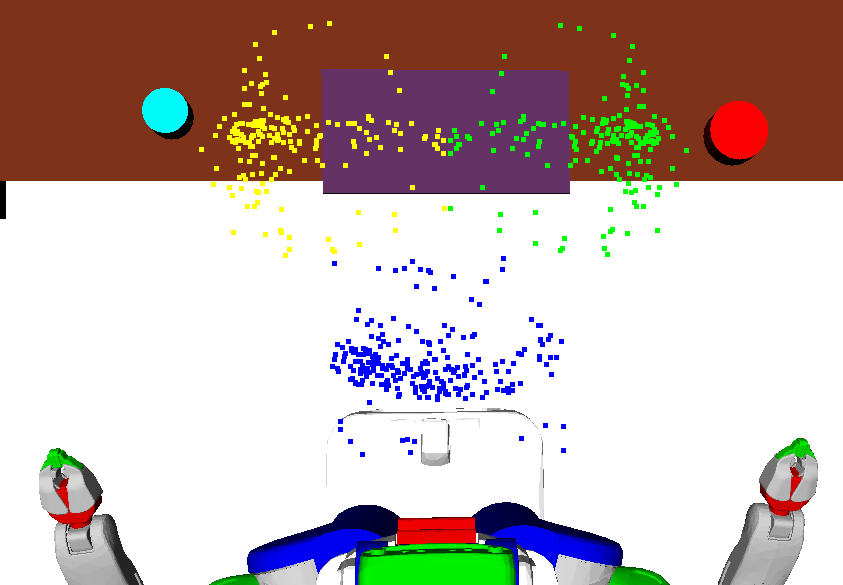
\includegraphics[width=\textwidth]{images/dinner_tray_final.png}
    \caption{Final distributions.}
  \end{subfigure}
  \caption{\small{Initial and learned base position (blue) and tray pickup (green, yellow) distributions
for the dinner domain. The green points refer to the position of the right tool center point; the gripper
is oriented toward the tray. The left gripper is placed in a symmetric position on the other side of
the tray, as marked by the yellow points. Final distributions are after 20 iterations.}}
  \label{fig:dinner}
\end{figure}

\subsection{Dinner Domain}
We run two sets of experiments, using 2 and 4 bowls. The robot must move the
bowls from their initial locations on one table to target locations on the other. We assign a cost to
base motion in the environment, so the robot is encouraged to use the provided tray, onto which bowls can be stacked.
This domain has 5 types of continuous references: base poses, object grasp poses, object putdown poses, tray pickup
poses, and tray putdown poses.

Our curriculum learning system first trains base poses and tray pickup and putdown poses for
$N = 20$ iterations, then object grasp and putdown poses for $N = 20$ iterations. We fixed $H = 100$ and $\epsilon = 10$.

The results demonstrate comparable performance to the baseline systems. The reason is that
hand-coding the sample space works well in this domain. For example, the optimal
robot base pose from which to pick up the tray is directly in front of it, which is quickly sampled in
the baseline systems. Additionally, the lack of long-term dependencies in the plan
means that backtracking search finds a valid refinement quickly. The fact that our system performs comparably
with the baselines shows that our algorithm can learn pose instantiations for a variety of objects.
\figref{fig:dinner} shows learned tray pickup poses.

\begin{figure}[t]
  \centering
  \begin{subfigure}[b]{0.25\linewidth}
    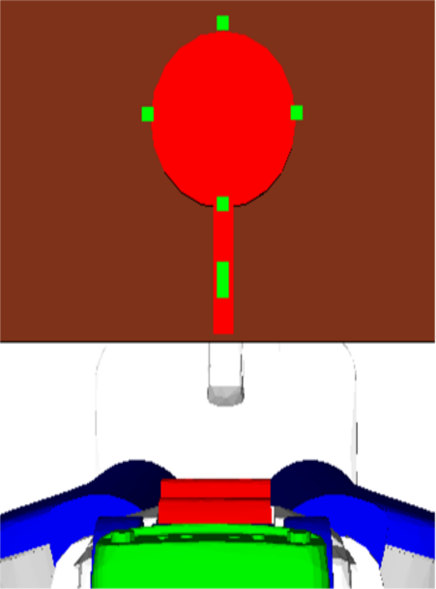
\includegraphics[width=\textwidth]{images/frying_hand.png}
    \caption{Hand-coded distribution.}
  \end{subfigure}
  \begin{subfigure}[b]{0.25\linewidth}
    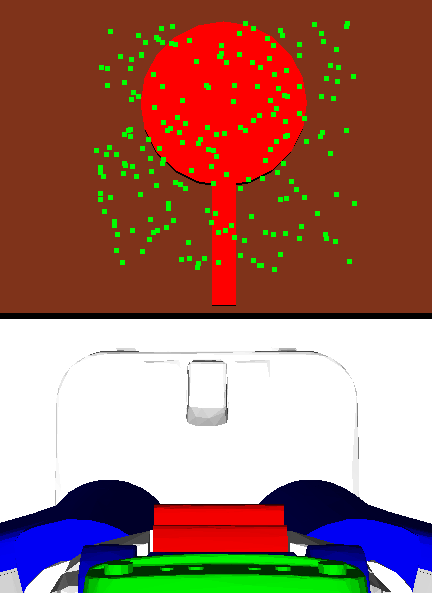
\includegraphics[width=\textwidth]{images/frying_initial.png}
    \caption{Initial distribution.}
  \end{subfigure}
  \begin{subfigure}[b]{0.25\linewidth}
    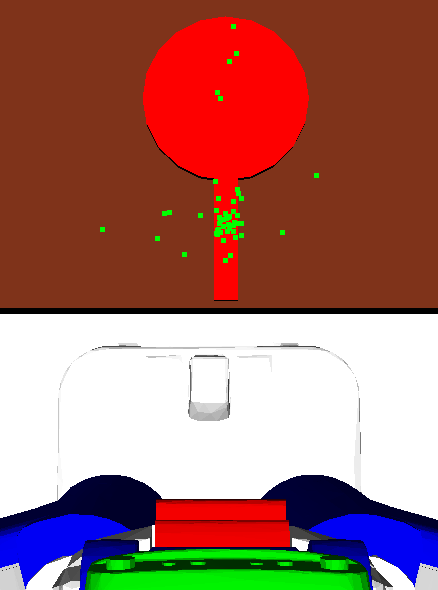
\includegraphics[width=\textwidth]{images/frying_final.png}
    \caption{Final distribution.}
  \end{subfigure}
  \caption{\small{Hand-coded distribution, along with initial and final distributions using our training methods,
for picking up the frying pan. The green points refer to the position of the tool center point; the end
effector is oriented downward. Our system learned to prefer picking up the pan at its handle to fit it into the shelf (not shown). Final distributions are after 20 iterations.}}
  \label{fig:frying}
\end{figure}

\subsection{Frying Domain}
We run two sets of experiments, using 2 and 4 frying pans. The robot must stack the frying pans in order of decreasing
radius into a narrow shelf. To be successful, it must grasp the frying pans at the handle, so that the handle sticks out
after the pan is placed in the shelf. This domain has 3 types of continuous references: base poses, pan grasp poses, and
pan putdown poses. We do not use curriculum learning, as weights for all these parameters can be trained jointly.
We fixed $N = 30$, $H = 100$, and $\epsilon = 5$. {\sc sfrcra-14} did not have a frying domain, so we used the following
hand-coded distribution for picking up the pans: 4 grasp poses in the cardinal directions around the lip of the pan,
and 4 grasp poses equidistant along the handle.

The results demonstrate significantly higher success rate versus the baseline systems. The backtracking baseline is faster likely because
the refinement times were averaged over cases where all 3 systems succeeded; backtracking often succeeded only when
it ``got lucky'' and picked grasp poses along the handle early in the search. \figref{fig:frying} compares the hand-coded
distribution with one we learned for picking up a frying pan.